\section{\ttbar control region} \label{sec:background:ttbar}

The substantial contribution to the SR by boosted $t\bar{t}$ shown in
\Cref{table:efficiencies_and_yields} makes its modeling a top
priority~\footnote{Pun!}.  Unfortunately, current MC generators are not able to
predict the $t\bar{t}$ cross section well in this boosted regime as seen in
\Cref{sec:background:mismodeling}.  This long-standing issue is likely due to
missing higher order diagrams rather than due to suboptimal generator setup
\cite{ATL-PHYS-PUB-2018-009}.  To compensate for this mismodeling the
$t\bar{t}$ yield in the SR is corrected with a normalization scale factor.  The
scale factor, or $k$-factor, is derived by fitting the $t\bar{t}$ normalization
of the in the $t\bar{t}$ enriched control region ($\text{CR}_{t\bar{t}}$).  In
the final fit the SR $t\bar{t}$ MC sample is fit by a double-sided crystal ball
function \cite{Gaiser:1982yw} to smooth out statistical fluctuations.  Its
normalization is constrained with the derived $k$-factor using its uncertainty
as the width of the gaussian prior.

\begin{figure}[!htbp]
\centering
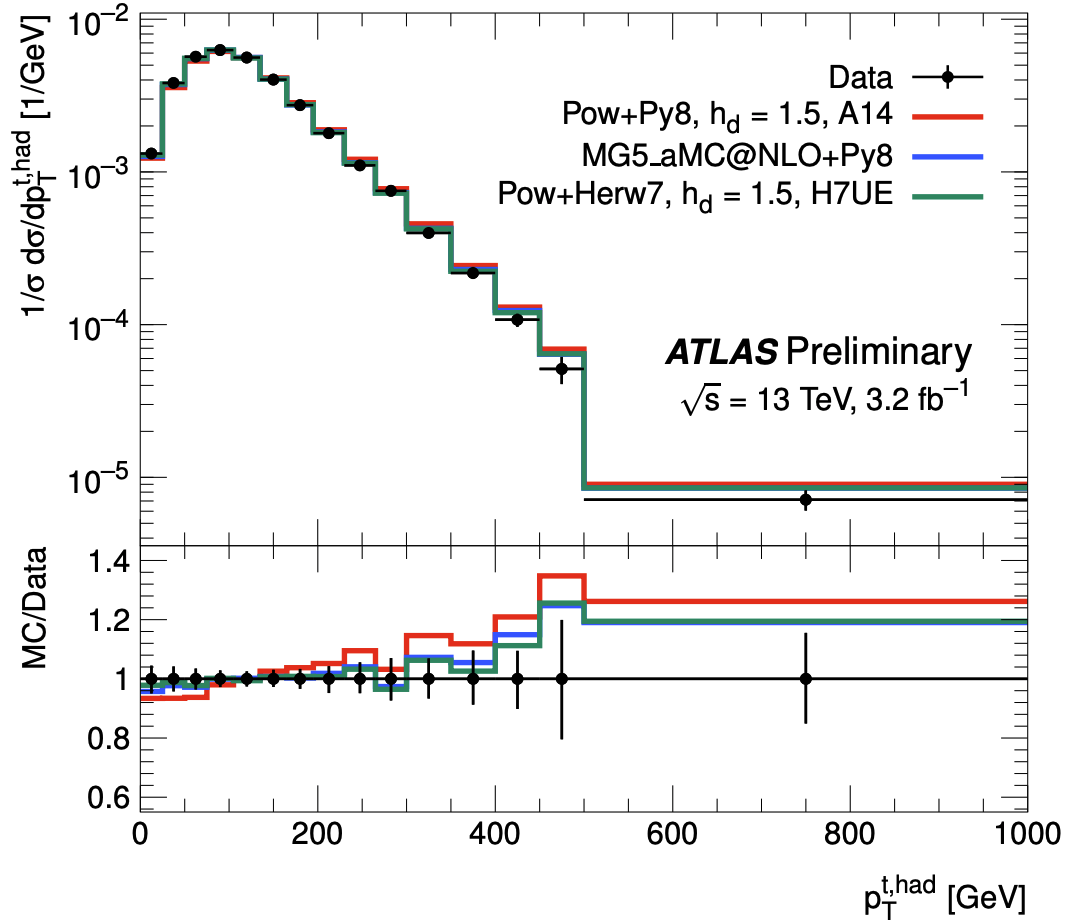
\includegraphics[width=0.6\linewidth]{figures/backgrounds/mismodeling}
\caption{Comparison in $p_{T}$ of the top quark for diffferent generator setups
used to assess the NLO+PS matching as well as the parton shower and
hadronisation uncertainty after optimisation, compared to data at $\sqrt{s} =
13~\TeV$.}
\label{sec:background:mismodeling}
\end{figure}

\subsection{Constructing $\text{CR}_{t\bar{t}}$}

The $t\bar{t}$ enriched control region uses the same $p_{T}$ selections as the
signal candidate large-$R$ jet in addition to the following criteria to select
$t\bar{t}$ events like the one shown in \Cref{sec:background:ttbar_depiction}.
Three regions are defined by requiring zero ($\text{CR}_{t\bar{t}0}$), one
($\text{CR}_{t\bar{t}}$) or two ($\text{CR}_{t\bar{t}2}$) tight quality
$b$-tags in the two leading VR track jets of the signal candidate. The
configuration with exactly one $b$-tag ,$\text{CR}_{t\bar{t}}$, is was chosen
to exploit the single $b$-quark that results from the dominant decay mode of
the top quark $t \rightarrow bW$.  The other two regions are used to validate
the extrapolation of the $k$-factor into the $\text{CR}_{\text{QCD}}$ and SR.

\begin{figure}[!htbp]
  \centering
\subcaptionbox{\label{sec:backgrounds:ttbar_feynman}}{
\resizebox{0.48\linewidth}{!}{
\begin{tikzpicture}
  \begin{feynman}
    % initial state particles
    \vertex (i1) {\(q\)};
    \vertex [below=2cm of i1] (i2) {\(q\)};

    % vertices
    \vertex [below right=1.cm and 1cm of i1] (a);
    \vertex [right=0.7cm of a] (b);

    % final state particles
    \vertex [above right=0.3cm and 0.5cm of b] (t1);
    \vertex [below right=0.3cm and 0.5cm of b] (t2);

    \vertex [above right=0.7cm and 0.7cm of t1] (W1);
    \vertex [blue, right=1.0cm of t1] (f1) {\(b\)};

    \vertex [blue, right=1.0cm of t2] (f2) {\(b\)};
    \vertex [below right=0.7cm and 0.7cm of t2] (W2);

    \vertex [above right=0.1cm and .6cm of W1] (f3) {\(\mu\)};
    \vertex [below right=0.1cm and .6cm of W1] (f4) {\(\nu_{\mu}\)};
    \vertex [above right=0.1cm and .6cm of W2] (f5) {\(q\)};
    \vertex [below right=0.1cm and .6cm of W2] (f6) {\(q\)};

    \diagram* {
      (i1) -- [fermion] (a) 
        -- [fermion] (i2),

      (a) -- [gluon, edge label'=\(g\)] (b),

      (t1) -- [orange, fermion, edge label'=\(t\)] (b)
        -- [orange, fermion, edge label'=\(t\)] (t2),

      (f1) -- [blue, fermion] (t1)
        -- [red, boson, edge label=\(W\)] (W1),
      (f2) -- [blue, fermion] (t2)
        -- [red, boson, edge label'=\(W\)] (W2),

      (f3) -- [fermion] (W1)
        -- [fermion] (f4),
      (f5) -- [fermion] (W2)
        -- [fermion] (f6),
    };

      
  \end{feynman}
\end{tikzpicture}
}} \hfill
\subcaptionbox{\label{sec:backgrounds:ttbar_cartoon}}{
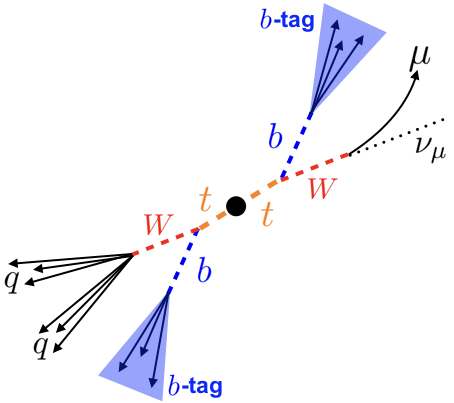
\includegraphics[width=0.48\linewidth]{figures/backgrounds/ttbar_cartoon}
}

\caption{(a) Feynman diagram of $t\bar{t}$ decay to $b$-quarks and semi-leptonic $W$-boson decays. (b) Cartoon depticting $t\bar{t}$ decay to $b$-quarks and semi-leptonic $W$-boson decays in center of mass frame.}
\label{sec:background:ttbar_depiction}

\end{figure}

To reduce QCD containation in the sample the second top quark in the opposite
hemisphere of the signal candidate is required to decay semileptonically in the
muon channel. \Cref{sec:backgrounds:phi_study} compares the $\Delta\phi$
between the leading muon in the event and the signal candidate for the QCD and
$t\bar{t}$ MC samples. This distribution shows the expected back-to-back
topology of the $t\bar{t}$ depicted in \Cref{sec:backgrounds:ttbar_cartoon}
versus the QCD sample where the muons are mostly produced close to the signal
candidate from hadron decays in flight. Thus, a cut of $\Delta\phi(muon-signal)
> \frac{2\pi}{3}$ was chosen to reduce the QCD contribution by several orders
of magnitude while only reducing the $t\bar{t}$ contribution by roughly a
factor of three~\footnote{This is expected as the leptonic decay of $W$ is mostly
agnostic to lepton flavor giving them roughly uniform branching fractions,
$BR(W \rightarrow \mu \nu_{mu}) / BR(W \rightarrow l \nu_l) = \frac{1}{3}$.}.

The QCD contribution is further suppressed using a cut on the muon $p_{T}$.
\Cref{sec:backgrounds:pt_study} compares the $p_{T}$ spectra for $t\bar{t}$ and
QCD before the $\Delta\phi$ cut selection. The boost and larger mass of the $W$
boson lead to higher $p_{T}$ muons than the softer QCD initiated muons.

\begin{figure}[!htbp]
\centering
\subcaptionbox{$\Delta \phi(\text{leading muon}-\text{signal})$ study \label{sec:backgrounds:phi_study}}{
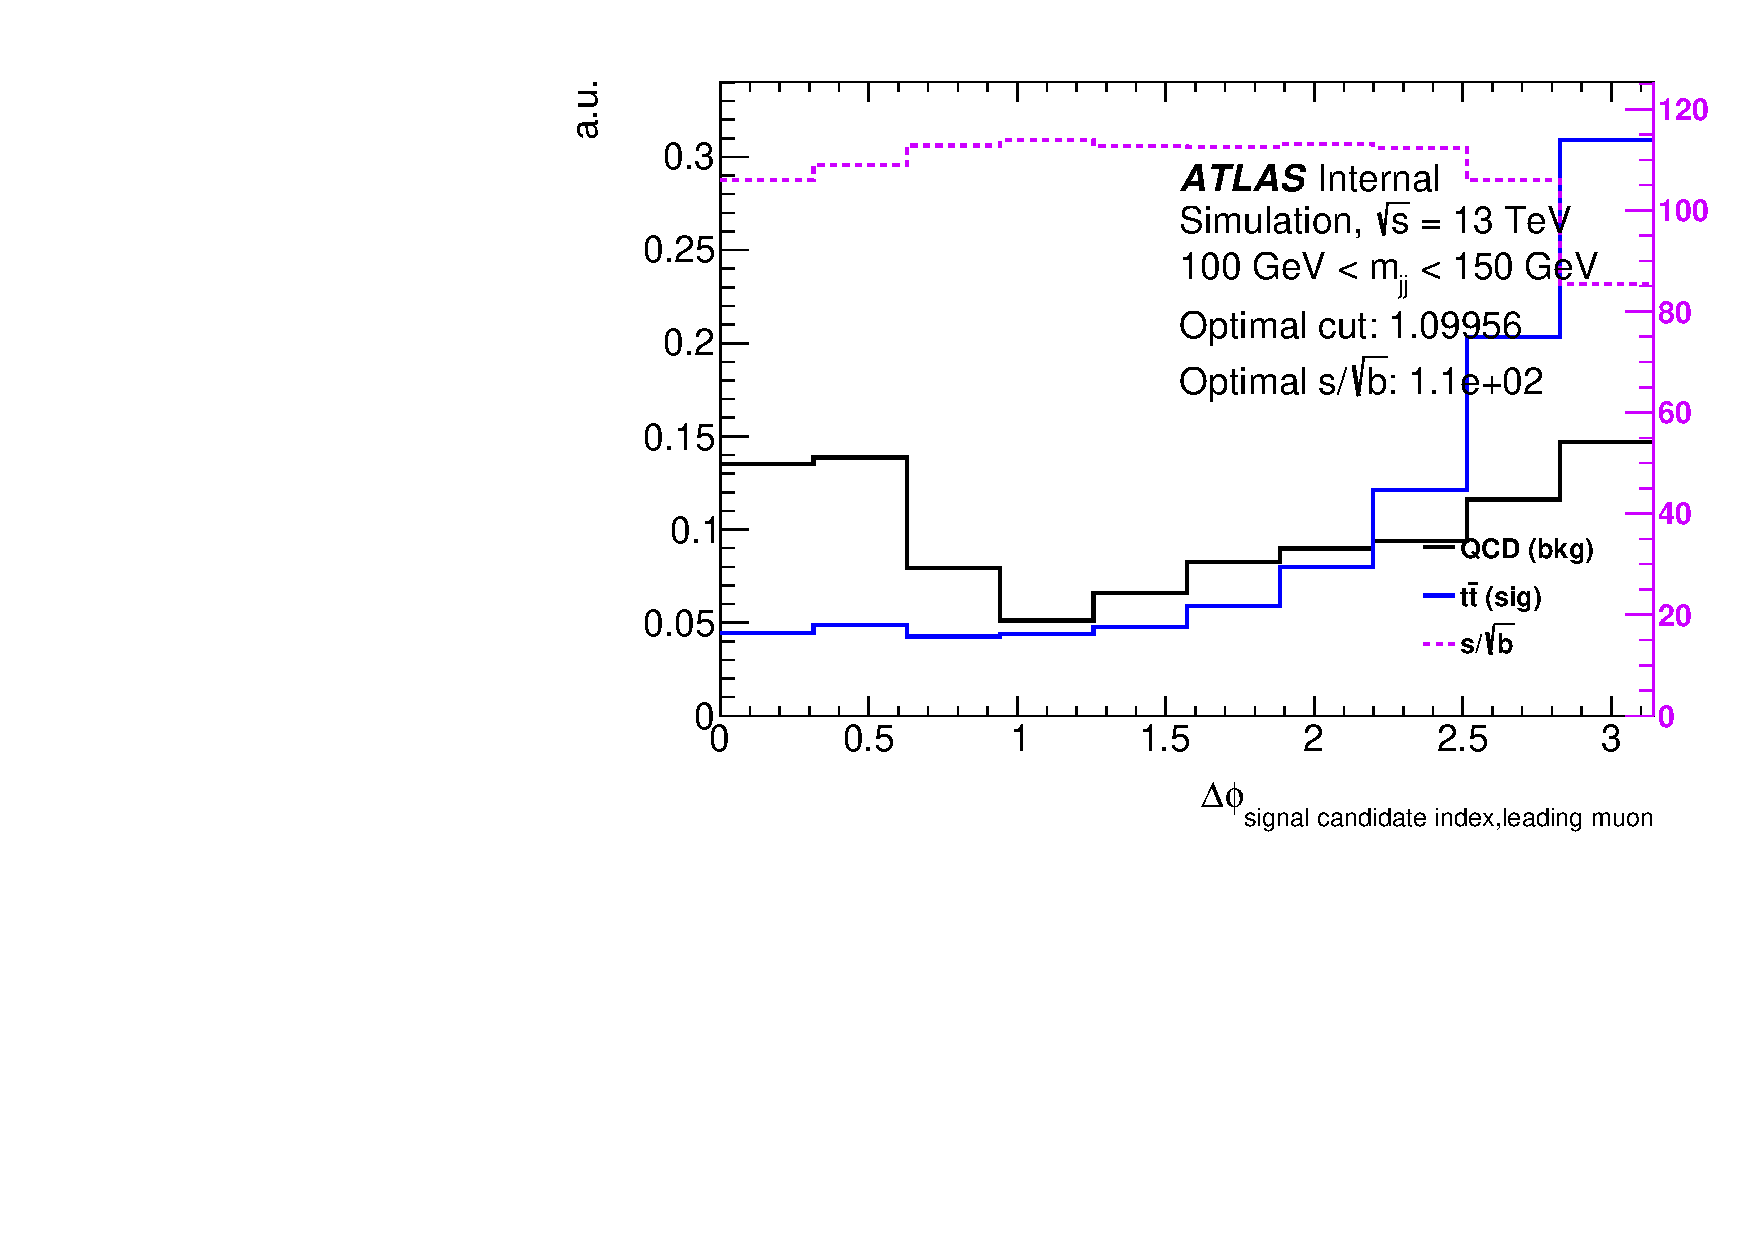
\includegraphics[width=0.48\linewidth]{figures/backgrounds/phi_study}
}\hfill
\subcaptionbox{Leading muon $p_{T}$ study \label{sec:backgrounds:pt_study}}{
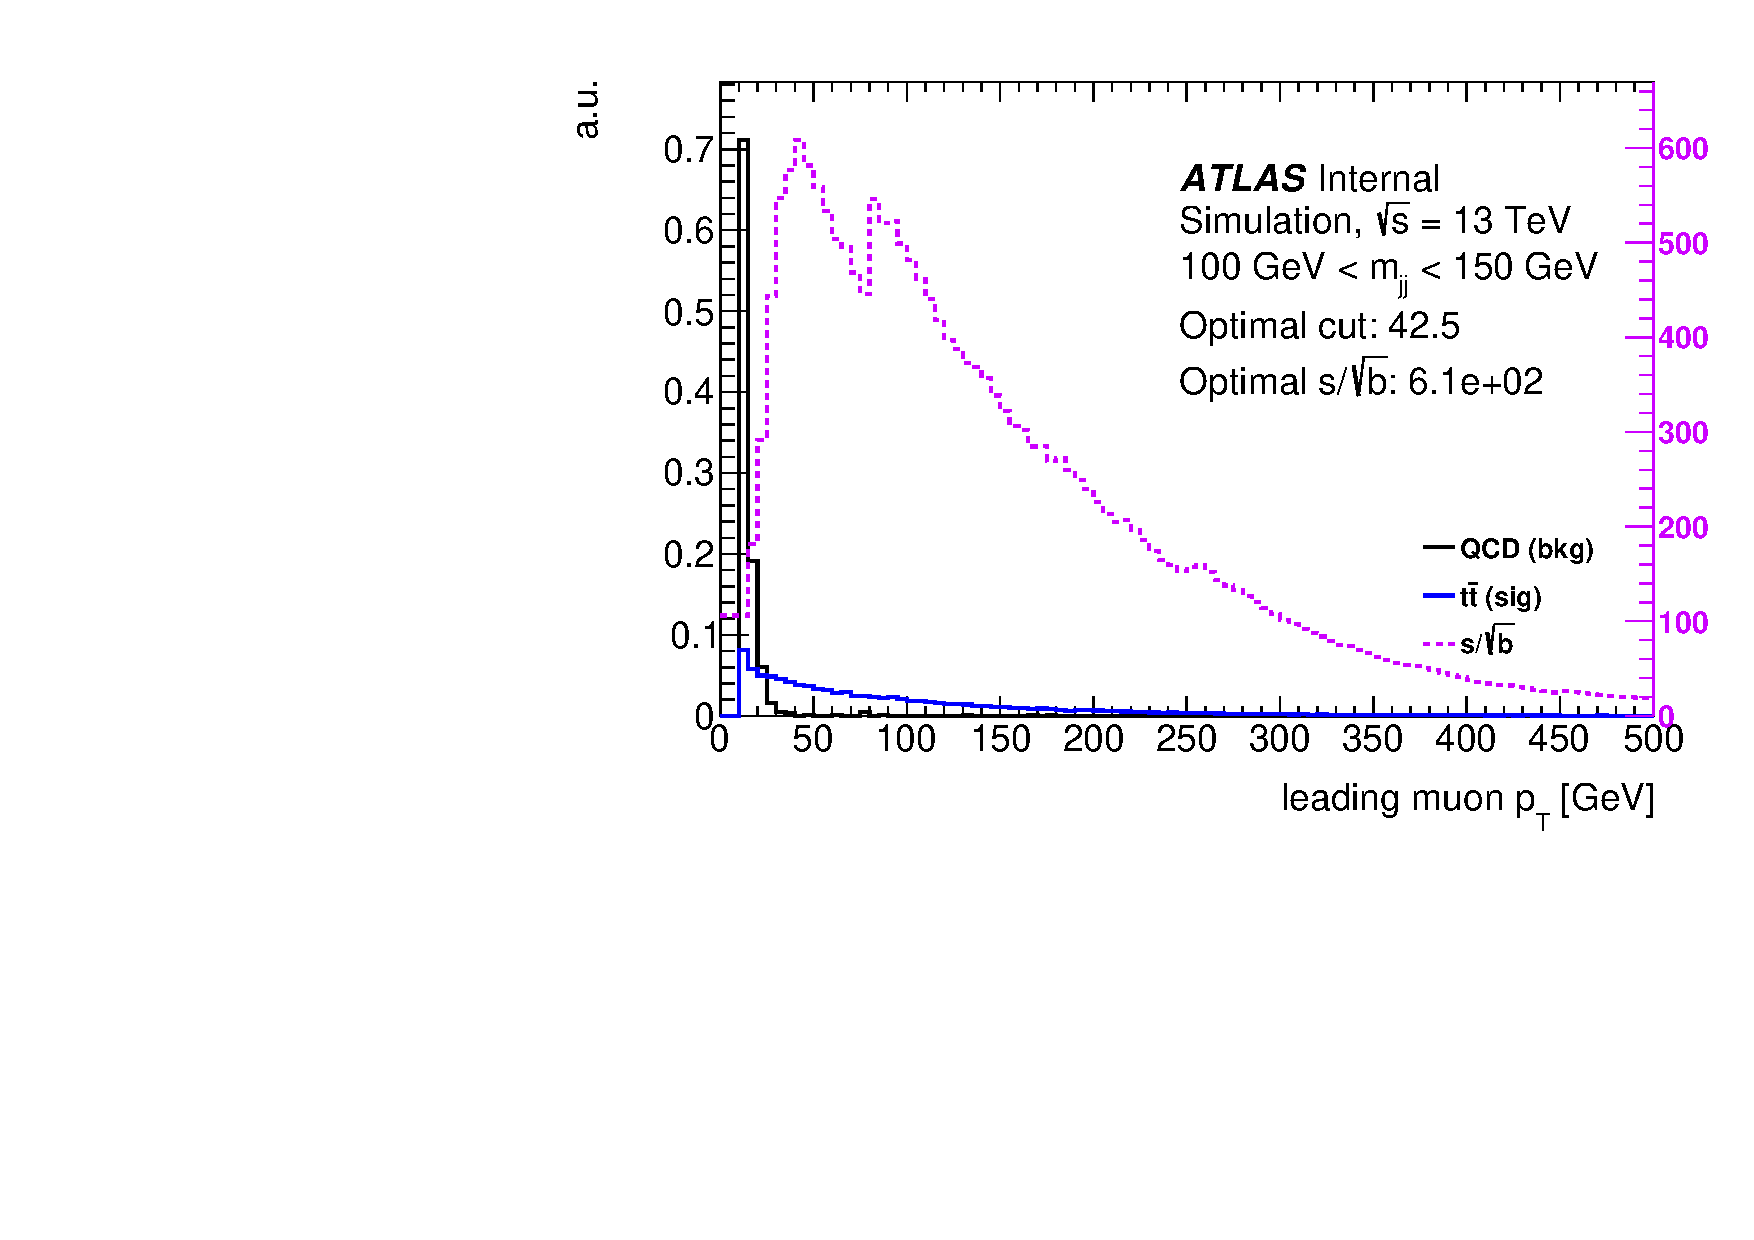
\includegraphics[width=0.48\linewidth]{figures/backgrounds/pt_study}
}
\caption{Comparison of the two variables, $\Delta \phi(\text{leading muon}-\text{signal})$ (a) and muon $p_{T}$ (b), between \textsc{Pythia}8 QCD and \textsc{Powheg} \ttbar simulated events used to create the \ttbar control region. The selection requires exactly one b-tagged track jet in the signal candidate \largeR jet. The magenta line shows the $s/\sqrt{b}$ significance with $80.5 \text{fb}^{-1}$.}
\label{sec:background:qcd_rejection_studies}
\end{figure}

Finally, at least one tight $b$-tagged track-jet is required to be within
$\Delta R < 1.5$ of the chosen muon.  This requirement exploits the collimation
of the semi-leptonic decay products of the boosted top quark $t \rightarrow
b\mu\nu_{\mu}$.  This requirement reduces the contamination from $V(ll)$+jets
and $VV$ events. The above $\text{CR}_{t\bar{t}}$ requirements are summarized visually in \Cref{sec:background:ttbar_selection_diagram}.

\begin{figure}[!htbp]
\centering
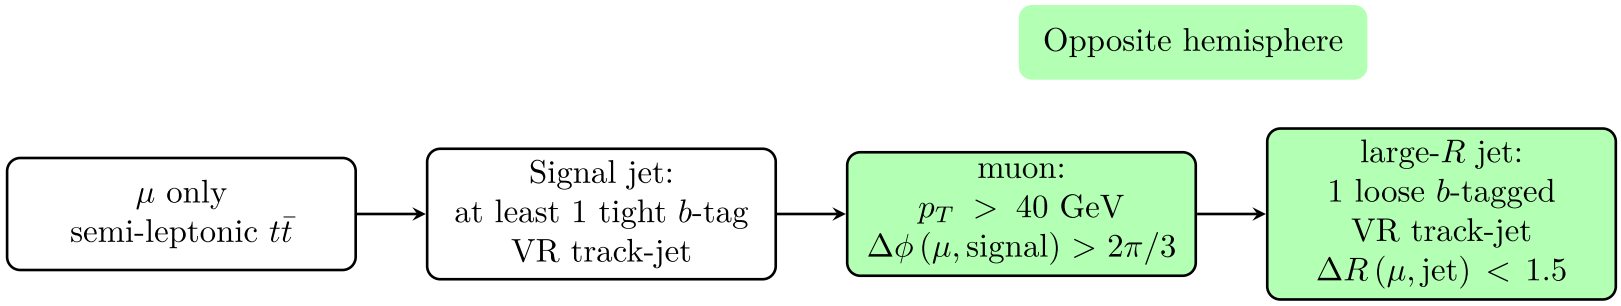
\includegraphics[width=1.0\linewidth]{figures/backgrounds/ttbar_selection}
\caption{\cite {Feickert:2690521} Diagram of the $\text{CR}_{t\bar{t}}$ selection criteria.}
\label{sec:background:ttbar_selection_diagram}
\end{figure}

\subsection{$k$-factor Estimation}

Finally the $t\bar{t}$ MC template is fit to the data in the
$\text{CR}_{t\bar{t}}$ over the mass range $100~\GeV$ to $200~\GeV$.  Single
top ($Wt$) and $W \rightarrow l\nu$ templates were included in the fit with
their normalizations kept constant. The full statistical and systematic
uncertainty is determined by running the Bayesian Analysis Toolkit
\cite{Beaujean:2011zz}, discussed in \Cref{chap:fit}, with the large-$R$ jet
energy scale (JES), jet mass resolution (JMR), luminosity, $t\bar{t}$
modeling and flavor tagging nuisance parameters discussed in
\Cref{chap:systematics}.

The pre- and post-fit distributions for the $\text{CR}_{t\bar{t}}$ are shown in
\Cref{sec:background:ttbar_fit} with the pull distributions shown in
\Cref{sec:background:ttbar_pulls}.  The JES and JMR systematics are constrained
by information about the peak in $t\bar{t}$ which was not available in the
dataset used to derive the recommendations. A $k$-factor of $0.84 \pm 0.11$ is
found for $\text{CR}_{t\bar{t}}$, showing that the MC overestimates the
$t\bar{t}$ yield as expected (see \Cref{sec:background:mismodeling}). This
value is used to constrain the $t\bar{t}$ contribution in the final fit to the
SR. The results for all three $t\bar{t}$ control regions are given in
\Cref{table:ttbar_kfactors}.  All three regions are consistent with eachother
and the results of the dedicated boosted top quark study presented in reference
\cite{ATLAS:2016jct}.

\begin{table}
  \centering
  \caption{The \ttbar scale factors and their uncertanties from the three \ttbar
control regions. The value for CRttbar is used in the Signal Region. NOTE:
CRttbar2 fit failed due to low statistics but is almostly completely dominated
by ttbar in this region.  The value here is the simple ratio of nevents in ttbar
vs. data and the uncertainty is the ttbar statistical uncertainty.}
  \begin{tabular}{@{}lrr@{}}
    \toprule
    Region & scale factor & uncertainty \\
    \midrule
    CRttbar0 & $0.87$ & $0.12$ \\
    CRttbar  & $0.84$ & $0.11$ \\
    CRttbar2 & $0.96$ & $0.21$ \\
    \bottomrule
  \end{tabular}
  \label{table:ttbar_kfactors}
\end{table}

\begin{figure}[!htbp]
\centering
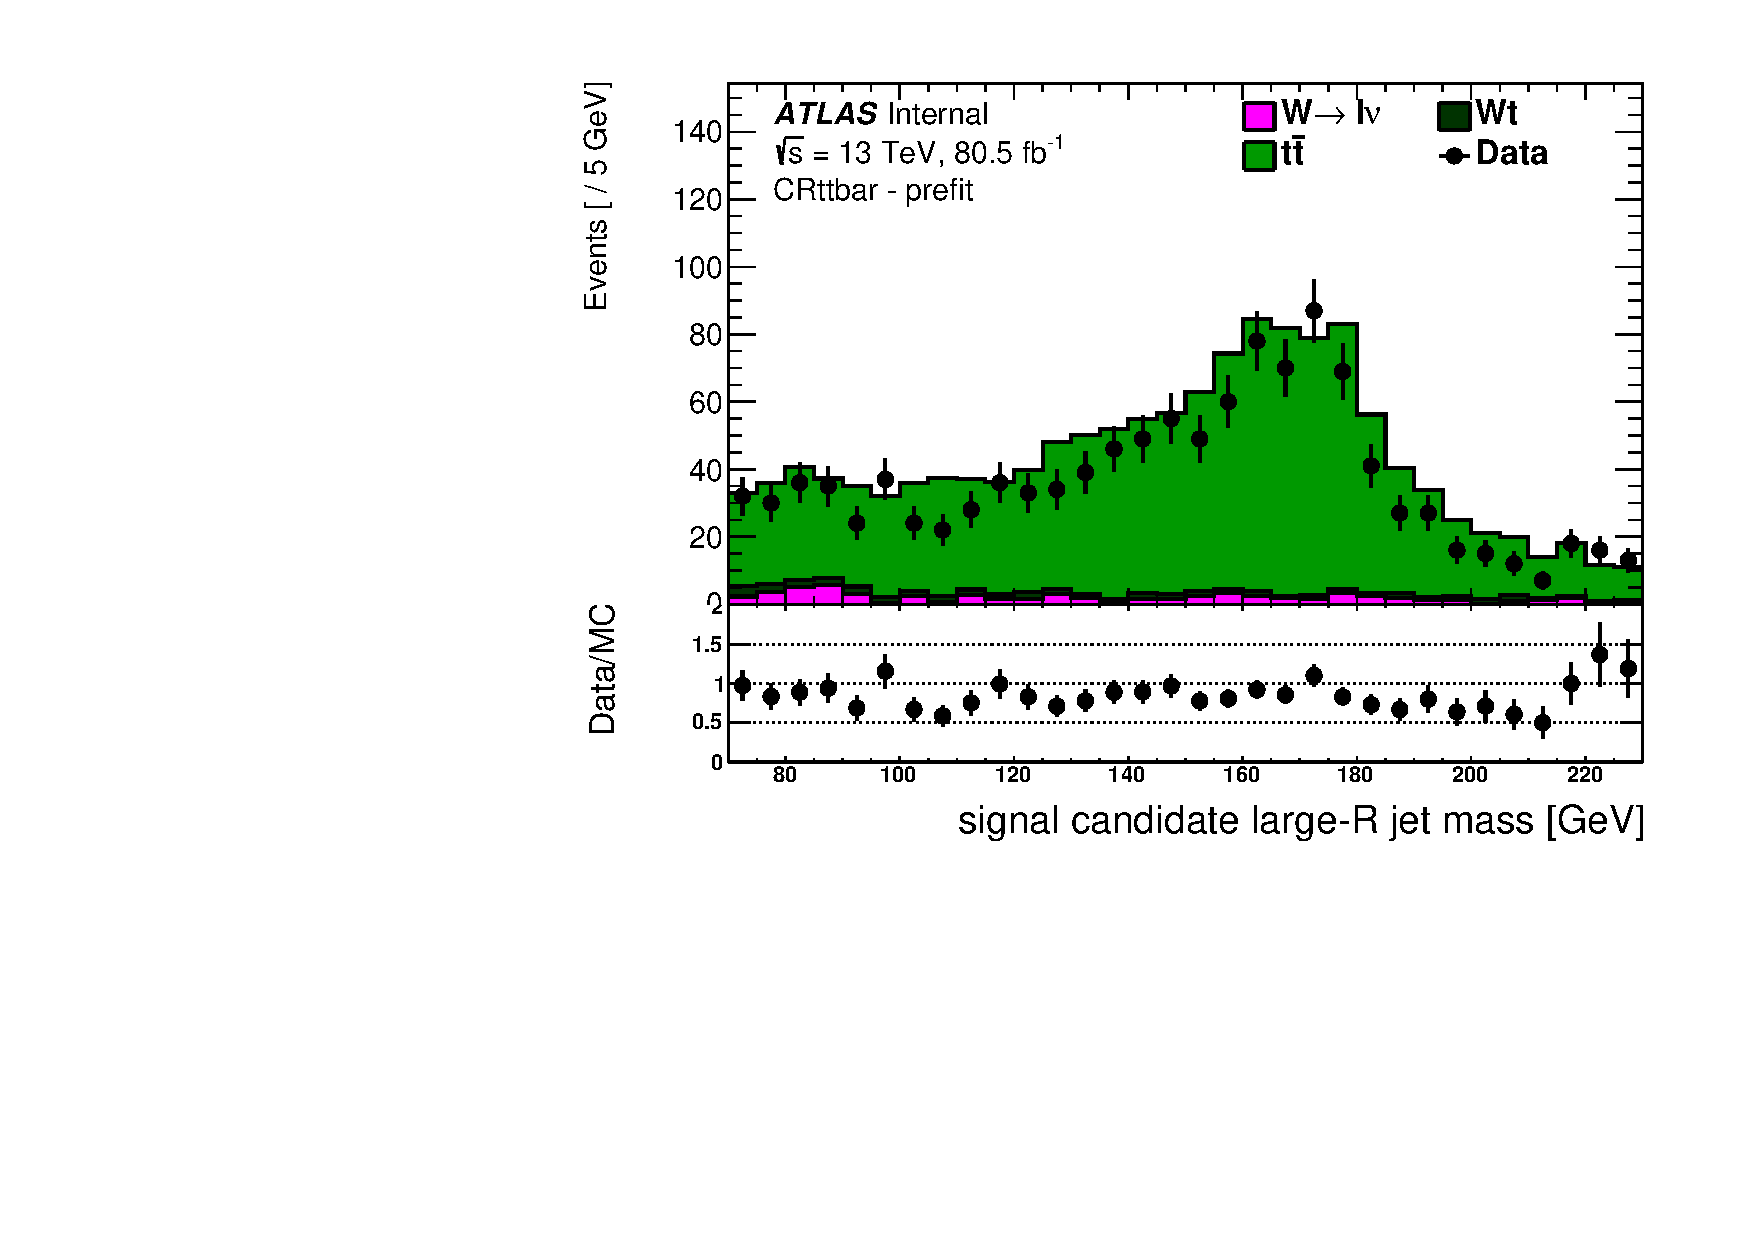
\includegraphics[width=0.49\linewidth]{figures/backgrounds/ttbar_prefit} \hfill
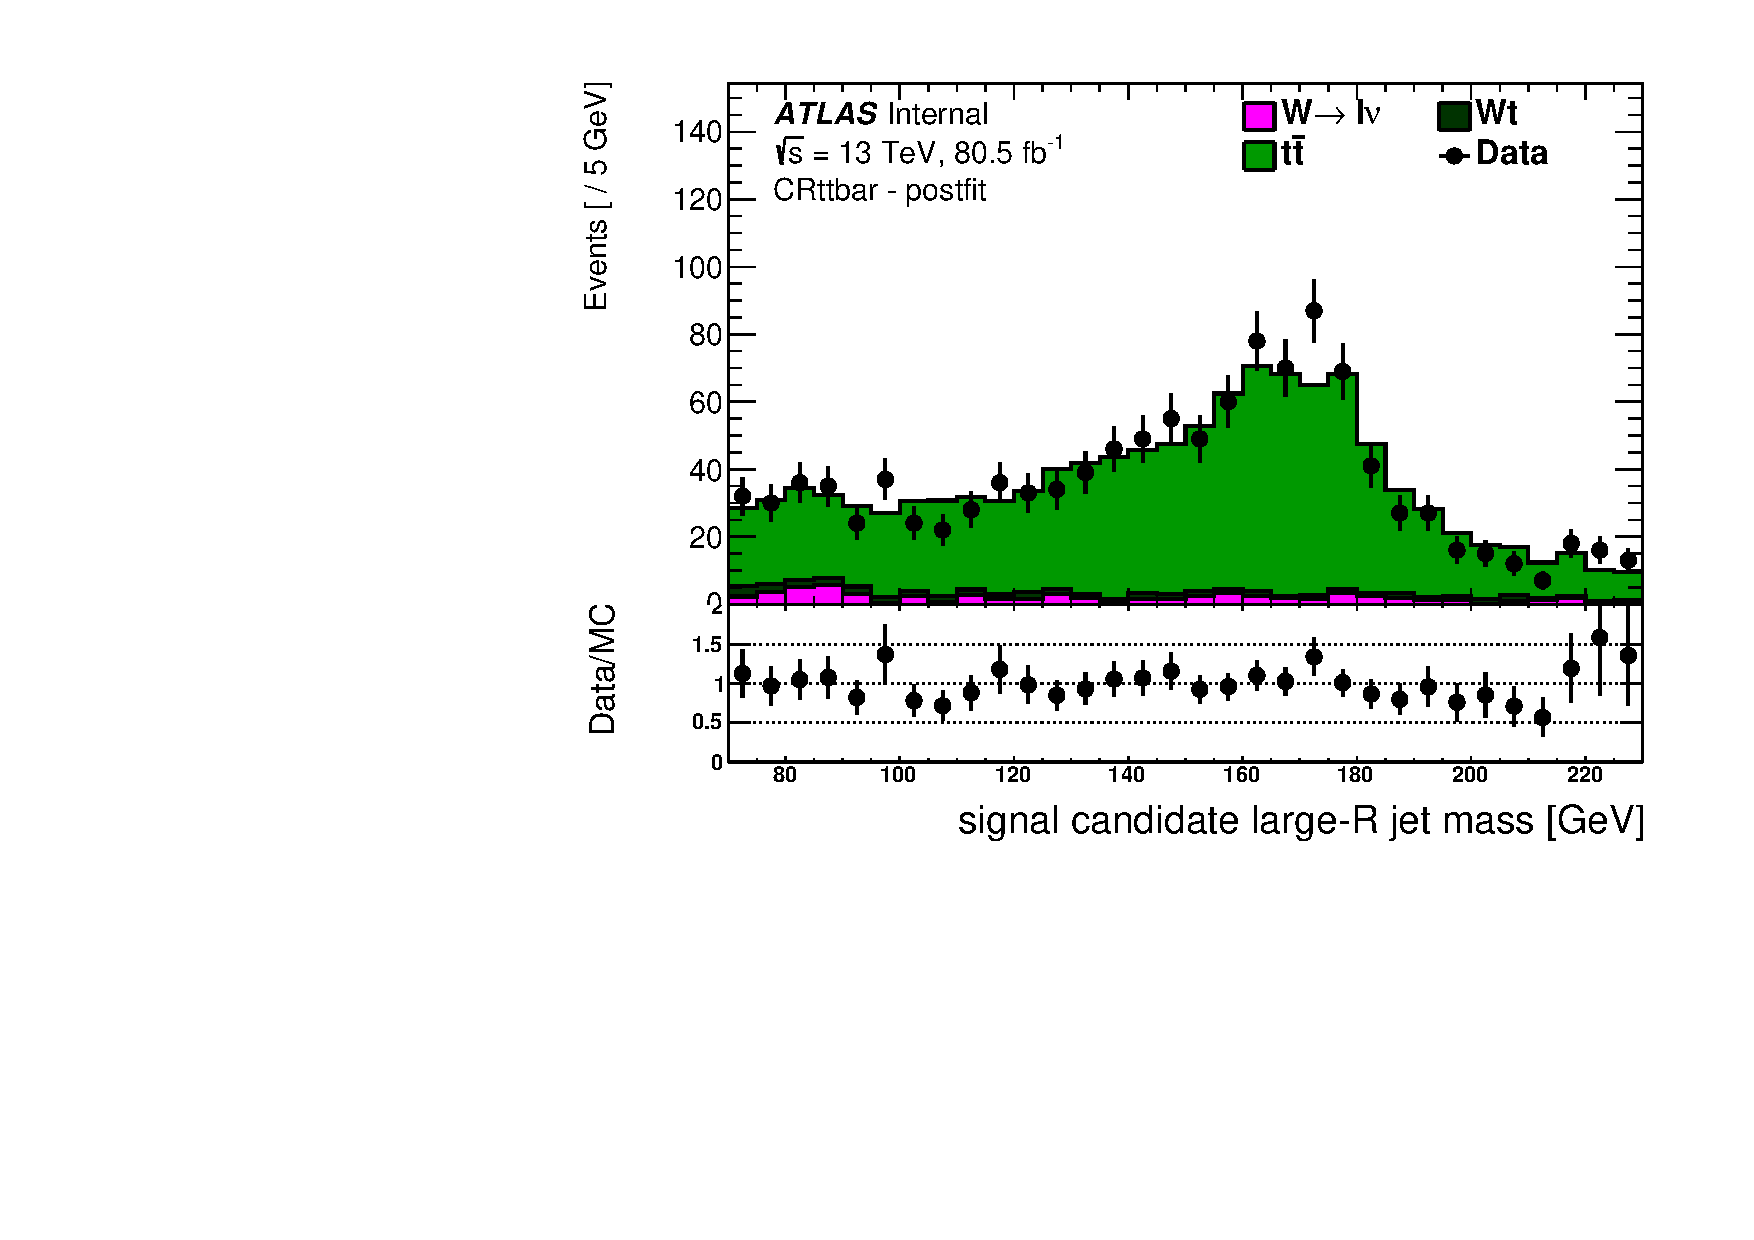
\includegraphics[width=0.49\linewidth]{figures/backgrounds/ttbar_postfit}
\caption{The pre-fit (left) and post-fit (right) data vs MC comparion for fitting the $\text{CR}_{t\bar{t}}$ region.}
\label{sec:background:ttbar_fit}
\end{figure}

\begin{figure}[!htbp]
\centering
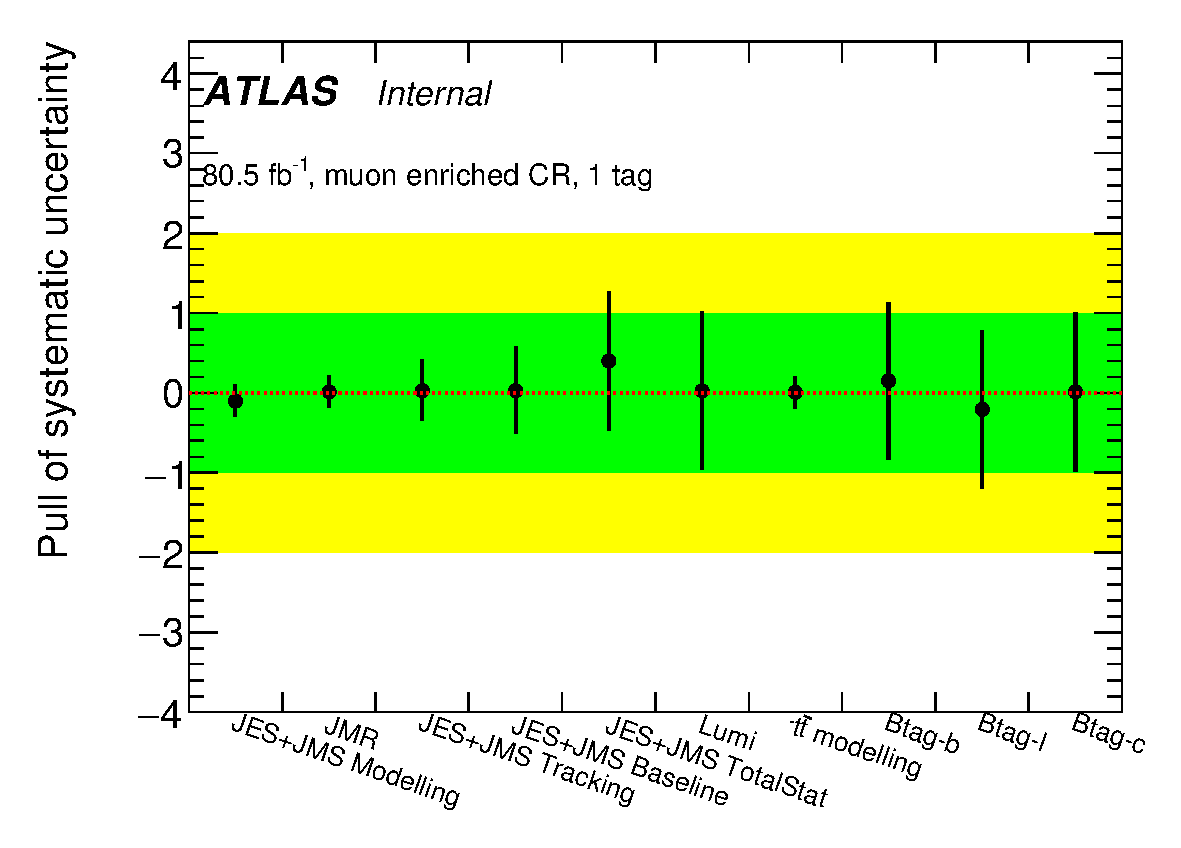
\includegraphics[width=0.7\linewidth]{figures/backgrounds/ttbar_pulls}
\caption{The pull distributions for the different nuisance parameters used in the $\text{CR}_{t\bar{t}}$ fit.}
\label{sec:background:ttbar_pulls}
\end{figure}
